\section{choosing sound classes}
in this chapter what sound that have been chosen to work with will be described based on research. Spectrograms of the sounds will be displayed to give a idea of how the sounds look like and how they differ.\\
the 3 sound that was chosen are based on some of the articles that have been read, where they have chosen similar sound\citep{Stowell2010}\citep{QBBB}. the sounds that have been used was the kick drum / bass drum, the snare drum and the high hat beat boxing sound.\\
\begin{figure}[h]
	\begin{center}
		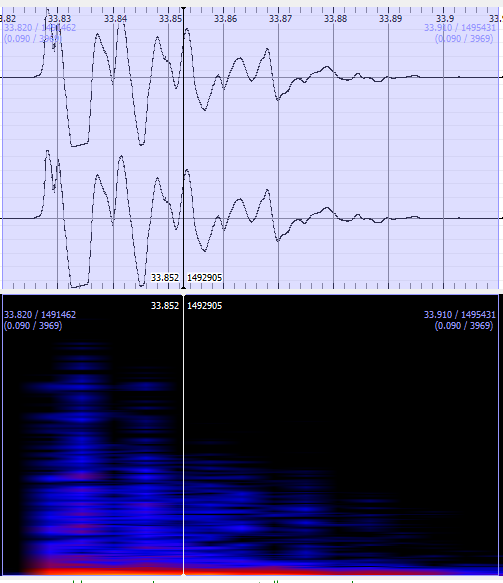
\includegraphics[scale = 0.5]{fig/Kick-closeup-with-spectrogram.png}
		\caption{kick sound in waveform and in spectrogram(low frequency in the bottom of the spectrogram and high frequency in the top), made with sonic visualizer}
		\label{KickCloseup}
	\end{center}
\end{figure} 
what can be seen on figure \ref{KickCloseup} is the kick sound, one can see that the kick sound has low frequency because the wave do not cross the 0 line that often and in the spectrogram one can seen more color in the bottom which is the low frequency.\\ 
\begin{figure}[h]
	\begin{center}
		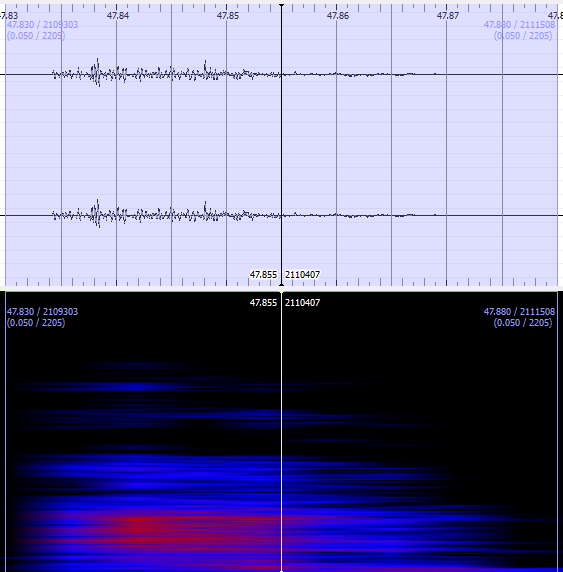
\includegraphics[scale = 0.5]{fig/Snare-close-up-with-spectrogram.png}
		\caption{snare sound in waveform and in spectrogram(low frequency in the bottom of the spectrogram and high frequency in the top), made with sonic visualizer}
		\label{snareCloseup}
	\end{center}
\end{figure}
on figure \ref{snareCloseup} we can see the a close up at the waveform of the snare sound, what we can see it that the sound has higher frequency on the spectrogram has more color closer to the top. 
\\
\begin{figure}[h]
	\begin{center}
		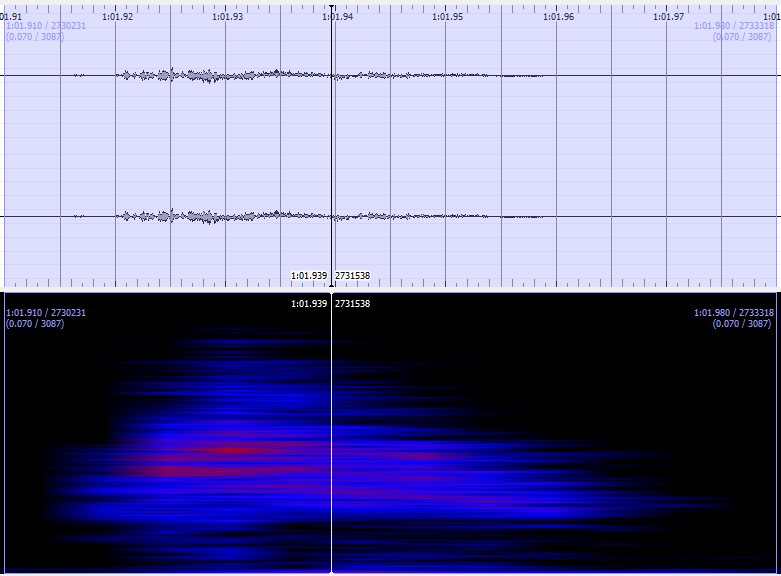
\includegraphics[scale =  0.5]{fig/HH-close-up-with-spectrogram.png}
		\caption{High Hat sound in waveform and in spectrogram(low frequency in the bottom of the spectrogram and high frequency in the top), made with sonic visualizer}
		\label{HHCloseup}
	\end{center}
\end{figure}
the last sound we have chosen for our transcription program is the high hat beat boxing sound, the high hat sound can be on figure \ref{HHCloseup} and it is possible to seen on this figure that the high hat also are in higher frequency than the kick drum beatboxing sound and also slightly higher than the snare drum for an easier compression of the 3 sounds one can look at figure \ref{HH-Snare-Kick}.
\begin{figure}[h]
	\begin{center}
		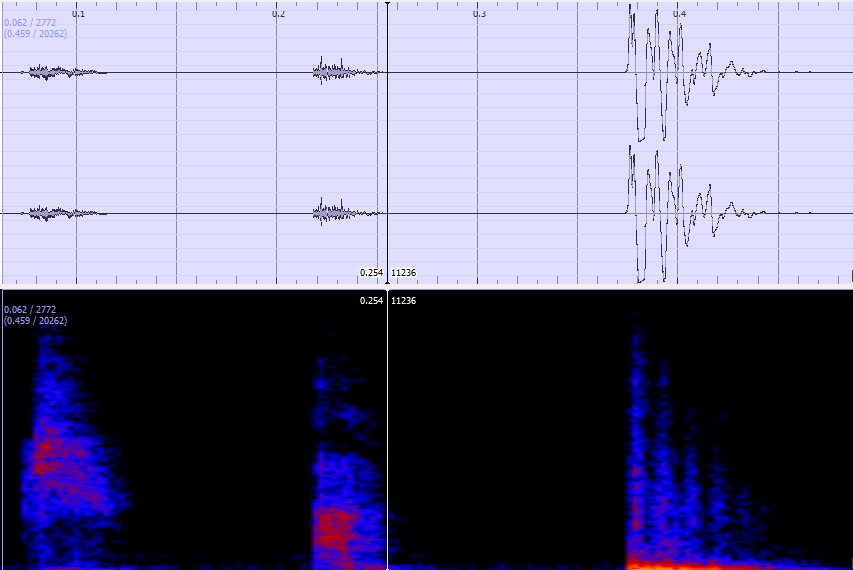
\includegraphics[scale =  0.5]{fig/hh-snare-kick-with-spectogram.png}
		\caption{High Hat, snare and kick sound in waveform and in spectrogram(low frequency in the bottom of the spectrogram and high frequency in the top), made with sonic visualizer}
		\label{HH-Snare-Kick}
	\end{center}
\end{figure}
what we can conclude from this is that the three sound look different with the greats different that the kick has compared to snare and high hat. in the waveform it is again the kick drum that will be most different.
